%%%%%%%%%%%%%%%%%%%%%%%%%%%%%%%%%%%%%%%%%%%%%%%%%%%%%%%%%%%%%%%%%%%%
\section{NMPC Problem Formulations}
%%%%%%%%%%%%%%%%%%%%%%%%%%%%%%%%%%%%%%%%%%%%%%%%%%%%%%%%%%%%%%%%%%%%
%%%%%%%%%%%%%%%%%%%%%%%%%%%%%%%%%%%%%%%%%%%%%%%%%%%%%%%%%%%%%%%%%%%%
\subsection{The NMPC Problem}
We consider a nonlinear discrete-time dynamic system expressed as \cite{economic}:
\begin{equation}
	\bf{x}_{k+1}=f(\bf{x}_k,\bf{u}_k)
	\label{eq:nonlin}
\end{equation}
where $\bf{x}_k\in\mathbb{R}^{n_x}$ denotes the state variable, $\bf{u}_k\in\mathbb{R}^{n_u}$ is the control input and $f:\mathbb{R}^{n_x}\times\mathbb{R}^{n_u}\rightarrow \mathbb{R}^{n_x}$ is a continuous model function, which calculates the next state $\bf{x}_{k+1}$ from the previous state $\bf{x}_k$ and control input $\bf{u}_k$, where $k\in\mathbb{N}$.
This system will be optimized by a nolinear model predictive controller which solves the problem:
	\begin{mini!}
		{\bf{z}_l,\bf{v}_l}{\boldsymbol{\Psi}(\bf{z}_N)+\sum_{l=0}^{N-1}\boldsymbol{\psi}(\bf{z}_l,\bf{v}_1)}{}{(\mathcal{P}_{NMPC}):}
		\addConstraint{\bf{z}_{l+1}}{=f(\bf{z}_l,\bf{v}_l),}{\qquad l=0,\ldots,N-1}
		\addConstraint{\bf{z}_0}{=\bf{x}_k}{}
		\addConstraint{(\bf{z}_l,\bf{v}_l)}{\in\mathcal{Z}}{}
		\addConstraint{\bf{z}_N}{\in\boldsymbol{\chi}_f}{}
	\end{mini!}
at each sample time.
Here $\bf{z}_l\in\mathbb{R}^{n_x}$ is the predicted state variable; $\bf{v}_l\in\mathbb{R}^{n_u}$ is the predicted control input; and $\bf{z}_n\in\boldsymbol{\chi}_f$ is the final predicted state variable restricted to the terminal region $\boldsymbol{\chi}_f\in\mathbb{R}^{n_x}$.
The stage cost is denoted by $\boldsymbol{\psi}:\mathbb{R}^{n_x}\times\mathbb{R}^{n_u}\rightarrow\mathbb{R}$ and the terminal cost by $\Psi:\boldsymbol{\chi}_f\rightarrow\mathbb{R}$.
$\mathcal{Z}$ denotes the path constraints where $\mathcal{Z}=\{(\bf{z},\bf{v})\;|\;q(\bf{z},\bf{v})\leq 0\}$, where $q:\mathbb{R}^{n_x}\times\mathbb{R}^{n_u}\rightarrow\mathbb{R}^{n_q}$.
The solution to this problem is denoted as $\{\bf{x}_0^*,\ldots,\bf{z}_N^*,\bf{v}_0^*,\ldots,\bf{v}_{N-1}^*\}$
\par
The idea is that at sample time $k$, an estimate or measurement of the state $\bf{x}_k$ is obtained and the problem $\mathcal{P}_{NMPC}$ is solved,
The first part of the optimal control sequence becomes the plant input such that $\bf{u}_k=\bf{v}_0^*$.
This part of the solution defines an implicit feedback law $\bf{u}_k=\boldsymbol{\kappa}(\bf{x}_k)$, and the system evolves according to Equation \ref{eq:nonlin}.
At the next sample time $k+1$, when the measurement of the new state is obtained, the procedure is repeated.
Algorithm \ref{alg:NMPC} summarizes the NMPC algorithm.\\
%FIX THIS FORMATTING
\begin{algorithm}[H]
	\SetAlgoLined
	set $k\leftarrow 0$\;
	\While{MPC is running}{
			Measure or estimate $x_k$.\\
			Assign the initial state: set $\bf{z}_0=x_k$.\\
			Solve the optimization problem $\mathcal{P}_{NMPC}$ to find $\bf{v}_0^*$.\\
			Assign the plant input $\bf{u}_k=\bf{v}_0^*$.\\
			Inject $\bf{u}_k$ to the plant.\\
			Set $k\leftarrow k+1$.\\
		}
	\caption{General NMPC algorithm.}
	\label{alg:NMPC}
\end{algorithm}
%%%%%%%%%%%%%%%%%%%%%%%%%%%%%%%%%%%%%%%%%%%%%%%%%%%%%%%%%%%%%%%%%%%%
%%%%%%%%%%%%%%%%%%%%%%%%%%%%%%%%%%%%%%%%%%%%%%%%%%%%%%%%%%%%%%%%%%%%
\subsection{Ideal NMPC and Advanced-Step NMPC Framework}
To achieve optimal economic performance and good stability properties, the problem shown in $\mathcal{P}_{NMPC}$ needs to be solved instantaneously, allowing the optimal input to be injected into the process without time delay.
This is known as ideal NMPC.
\par
In reality, there will always be some time delay between obtaining the updated values of the states and injecting them into the plant.
The main cause of this delay is the time required to solve the optimization problem $\mathcal{P}_{NMPC}$.
As the process models grow, so to does the computation time.
With sufficiently large systems, this computational delay cannot be neglected.
One approach is the advanced-step NMPC (asNMPC) which is based on the following steps:
\begin{enumerate}
	\item Solve the NMPC problem at time $k$ with a predicted state value of $k+1$
	\item When the measurement $\bf{x}_{k+1}$ becomes available at time $k+1$, compute an approximation of the NLP solution using fast sensitivity methods
	\item Update $k\leftarrow k+1$, and repeat from Step 1
\end{enumerate}
Different fast sensitivity methods can be used and are discussed further in Section \ref{sec:}.
%%%%%%%%%%%%%%%%%%%%%%%%%%%%%%%%%%%%%%%%%%%%%%%%%%%%%%%%%%%%%%%%%%%%
\section{Sensitivity-Based Path-Following NMPC}
Below we outline sensitivity results and then utilize them in a path-following scheme for obtaining fast approximate solutions to the NLP.
%%%%%%%%%%%%%%%%%%%%%%%%%%%%%%%%%%%%%%%%%%%%%%%%%%%%%%%%%%%%%%%%%%%%
%%%%%%%%%%%%%%%%%%%%%%%%%%%%%%%%%%%%%%%%%%%%%%%%%%%%%%%%%%%%%%%%%%%%
\subsection{Sensitivity Properties of NLP}
The dynamic optimization problem can be written as a generic NLP problem:
	\begin{mini}
		{\mathcal{X}}{F(\boldsymbol{\chi},\bf{p})}{\label{eq:param_NLP}}{(\mathcal{P}_{NLP}):}
		\addConstraint{c(\boldsymbol{\chi},\bf{p})}{=0}{}
		\addConstraint{g(\boldsymbol{\chi},\bf{p})}{\leq 0}{}
	\end{mini}
where $\boldsymbol{\chi}\in\mathbb{R}^{n_{\boldsymbol{\chi}}}$ are the decision variables (typically the state variables and the control input) and $\bf{p}\in\mathbb{R}^{n_p}$ is the parameter (typically the initial state variable).
$F:\mathbb{R}^{n_{\boldsymbol{\chi}}}\times \mathbb{R}^{n_p}\rightarrow\mathbb{R}$  is the scalar objective function, $c:\mathbb{R}^{n_{\boldsymbol{\chi}}}\times \mathbb{R}^{n_p}\rightarrow\mathbb{R}^{n_c}$ denotes the equality constraints, and $g:\mathbb{R}^{n_{\boldsymbol{\chi}}}\times \mathbb{R}^{n_p}\rightarrow\mathbb{R}^{n_g}$ denotes the inequality constraints.
Each instance of the general parameteric NLP shown in Equation \ref{eq:param_NLP} that are solved for each sample time differ only in the parameter $\bf{p}$.
\par
The Lagrangian function of this problem is defined as:
	\begin{equation}
		\Lagrange(\boldsymbol{\chi},\bf{p},\boldsymbol{\lambda},\boldsymbol{\mu}) = F(\boldsymbol{\chi},\bf{p})+\boldsymbol{\lambda}^Tc(\boldsymbol{\chi},\bf{p})+\boldsymbol{\mu}^Tg(\boldsymbol{\chi},\bf{p})
	\end{equation}
and the Karush-Kuhn-Tucker (KKT), first order optimality, conditions are written as \cite{economic}:
	\begin{align}
		c(\boldsymbol{\chi},\bf{p})&=0, \qquad g(\boldsymbol{\chi},\bf{p})\leq 0, \qquad \textit{(primal feasibility)}\label{eq:primal}\\
		\boldsymbol{\mu}&\geq0, \qquad\qquad\qquad\qquad\qquad\textit{(dual feasibility)}\nonumber\\
		\nabla_{\boldsymbol{\chi}}\Lagrange(\boldsymbol{\chi},\bf{p},\boldsymbol{\lambda},\boldsymbol{\mu}) &=0, \qquad\qquad\qquad\qquad\quad\textit{(stationary condition)}\nonumber\\
		\boldsymbol{\mu}^Tg(\boldsymbol{\chi},\bf{p})&=0, \qquad \qquad\qquad\qquad\textit{(complementary slackness)}\nonumber
	\end{align}
\par
For the KKT conditions to be a necessary condition of optimality we assume that the linear independence constraint qualification (LICQ) holds.
The LICQ states:
\begin{definition}{(LICQ)}
	Given a vector $\boldsymbol{p}$ and a point $\boldsymbol{\chi}$, the LICQ holds at $\boldsymbol{\chi}$ if the set of vectors $\bigg\{\{\nabla_{\boldsymbol{\chi}}c_i(\boldsymbol{\chi},\bf{p})\}_{i\in\{1,\ldots,n_c\}}\cup\{\nabla_{\boldsymbol{\chi}}g_i(\boldsymbol{\chi},\bf{p})_{i:g_i(\boldsymbol{\chi},\boldsymbol{p})=0}\}\bigg\}$
\end{definition}
This implies that the Lagrange multipliers $(\boldsymbol{\lambda},\boldsymbol{\mu})$ that satisfy the KKT conditions are unique.
If a second-order condition also holds then a unique local minimum is guaranteed.
The second-order condition states that the Hessian matrix must be positive definite in a set of appropriate directions defined in the following definition \cite{economic}:
\begin{definition}{(SSOSC)}
	The strong second-order sufficient condition (SSOSC) holds at $\boldsymbol{\chi}$ with multipliers $\boldsymbol{\lambda}$ and $\boldsymbol{\mu}$ if $\bf{d}^T\nabla_{\boldsymbol{\chi}}^2\Lagrange(\boldsymbol{\chi},\bf{p},\boldsymbol{\lambda},\boldsymbol{\mu})\bf{d}>0$ for all $\bf{d}\neq 0$, such that $\nabla_{\boldsymbol{\chi}}c(\boldsymbol{\chi},\bf{p})^T\boldsymbol{d}=0$ and $\nabla_{\boldsymbol{\chi}}g_i(\boldsymbol{\chi},\boldsymbol{p})^T\bf{d}=0$ for $i$, such that $g_i(\boldsymbol{\chi},\bf{p})=0$ and $\mu_i>0$.
\end{definition}
\par
One more important concept needs to be defined before sensitivity results can be discussed:
\begin{definition}{(SC)}
	Given a vector $\bf{p}$ and a solution $\boldsymbol{\chi}^*$ with vectors of multipliers $\boldsymbol{\lambda}^*$ and $\boldsymbol{\mu}^*$, strict complimentary (SC) holds if $\mu_i^*-g_i(\boldsymbol{\chi}^*,\bf{p})>0$ for each $i=1,\ldots,n_g$.
\end{definition}
\par
It has been shown by Fiacco \cite{sensitivity}:
\begin{theorem}{(Implicit function theorem applied to optimality conditions)}
	Let $\boldsymbol{\chi}^*(\bf{p})$ be a KKT point that satisfies Equation \ref{eq:primal}, and assumed that LICQ, SSOSC, and SC all hold at $\boldsymbol{\chi}^*$.
	Further, let the function $F,c,g$ be at least $k+1$-times differentiable in $\boldsymbol{\chi}$ and $k$-times differentiable in $\bf{p}$. Then:
	\begin{itemize}
		\item $\boldsymbol{\chi}^*$ is an isolated minimizer and the associated multipliers $\boldsymbol{\lambda}$ and $\boldsymbol{\mu}$ are unqiue
		\item for $\bf{p}$ in a neighborhood of $\bf{p}_0$, the set of active constraints remains unchanged
		\item for $\bf{p}$ in a neighborhood of $\bf{p}_0$, there exists a $k$-times differentiable function $\sigma(\bf{p})=\begin{bmatrix}\boldsymbol{\chi}^*(\bf{p})^T & \boldsymbol{\mu}^*(\bf{p})^T & \boldsymbol{\lambda}^*(\bf{p})^T\end{bmatrix}$, that corresponds to a locally unique minimum for Equation \ref{eq:param_NLP}
	\end{itemize}
\end{theorem}
\par
Using Fiacco's results, the sensitivity of the optimal solution $(\boldsymbol{\chi}^*, \boldsymbol{\lambda}^*,\boldsymbol{\mu}^*)$ in a small neighborhood of $\bf{p}_0$ can be found by solving the system of linear equations that arises from applying the implicit function theorem to the KKT conditions of Equation \ref{eq:param_NLP}:\\
%FIX FORMATTING (EQUATION NUMBER NOT ON SAME LINE)
	\begin{equation}
	%\mspace{-30mu}
	\raisetag{1\baselineskip}
	{\footnotesize
		\begin{bmatrix}
			\nabla_{\chi\chi}^2\Lagrange(\boldsymbol{\chi}^*,\bf{p}_0, \boldsymbol{\lambda}^*,\boldsymbol{\mu}^*) & \nabla_{\chi}(\boldsymbol{\chi}^*,\bf{p}_0)&\nabla_{\chi}g_A(\boldsymbol{\chi}^*,\bf{p}_0)\\
			\nabla_{\chi}c(\boldsymbol{\chi}^*,\bf{p}_0)^T & 0 & 0\\
			\nabla_{\chi}g_A(\boldsymbol{\chi}^*,\bf{p}_0)^T & 0 & 0
		\end{bmatrix}
		\begin{bmatrix}
			\nabla_{\bf{p}}\boldsymbol{\chi}\\
			\nabla_{\bf{p}}\boldsymbol{\lambda}\\
			\nabla_{\bf{p}}\boldsymbol{\mu}
		\end{bmatrix}
		=-
		\begin{bmatrix}
			\nabla_{\bf{p}\chi}\Lagrange(\boldsymbol{\chi}^*, \bf{p}_0,\boldsymbol{\lambda}^*,\boldsymbol{\mu}^*)\\
			\nabla_{\bf{p}}c(\boldsymbol{\chi}^*,\bf{p}_0)\\
			\nabla_{\bf{p}}g_A(\boldsymbol{\chi}^*,\bf{p}_0)
		\end{bmatrix}
	}
	\label{eq:sensitivity}
	\end{equation}
where $g_A$ indicates that only the vectors and components of the Jacobian corresponding to the active inequality constraints at $\boldsymbol{\chi}$ are included; in other words, where $i\in A$ if $g_i(\boldsymbol{\chi},\bf{p}_0)=0$.
\par
The solution to the system of the linear equations is written as $\begin{bmatrix}\nabla_{\bf{p}}\boldsymbol{\chi}&\nabla_{\bf{p}}\boldsymbol{\lambda}&\nabla_{\bf{p}}\boldsymbol{\mu}\end{bmatrix}^T$ it is possible to obtain a good estimate of the solution to the NLP problem for small $\Delta\bf{p}$ at the parameter value $\bf{p}_0+\Delta\bf{p}$:
	\begin{align}
		\boldsymbol{\chi}(\bf{p}_0+\Delta\bf{p})&=\boldsymbol{\chi}^*+\nabla_{\bf{p}}\boldsymbol{\chi}\Delta\bf{p}\\
		\boldsymbol{\lambda}(\bf{p}_0+\Delta\bf{p})&=\boldsymbol{\lambda}^*+\nabla_{\bf{p}}\boldsymbol{\lambda}\Delta\bf{p}\\
		\boldsymbol{\mu}(\bf{p}_0+\Delta\bf{p})&=\boldsymbol{\mu}^*+\nabla_{\bf{p}}\boldsymbol{\mu}\Delta\bf{p}
	\end{align}
However,  if $\Delta\bf{p}$ becomes large, the approximate solution may no longer be accurate enough because strict complementary requires that the active set cannot change.
This condition holds for small perturbations but may not necessarily hold for large changes in $\Delta\bf{p}$.
\par
Note that the sensitivity system of linear equations corresponds to the stationarity conditions for a particular QP \cite{economic}.
It can be proven that for $\Delta\bf{p}$ sufficiently small, the set $\{i\;:\;\boldsymbol{\mu}(\bar{\bf{p}})_i>0\}$ is constant for $\bar{\bf{p}}=\bf{p}_0+\Delta\bf{p}$.
A QP can then be formed where we move off weakly-active constraints but stay on the strongly-active ones.
The primal-dual solution of this QP will then be the directional derivative of the primal-dual solution path $\boldsymbol{\chi}^*(\bf{p}),\boldsymbol{\lambda}^*(\bf{p}),\boldsymbol{\mu}^*(\bf{p})$.

It has been shown that the perturbed NLP can be solved by solving a QP problem of the form \cite{perturb}:
\begin{mini}
	{\Delta\boldsymbol{\chi}}{\frac{1}{2}\boldsymbol{\chi}^T\nabla_{\boldsymbol{\chi}\boldsymbol{\chi}}^2\Lagrange(\boldsymbol{\chi}^*,\bf{p}_0,\boldsymbol{\lambda}^*,\boldsymbol{\mu}^*)\Delta\boldsymbol{\chi}+\Delta\boldsymbol{\chi}^T\nabla_{\bf{p}\boldsymbol{\chi}}^2\Lagrange(\boldsymbol{\chi}^*,\bf{p}_0,\boldsymbol{\lambda}^*,\boldsymbol{\mu}^*)\Delta \bf{p}}{}{\label{eq:QP}}
	\addConstraint{\nabla_{\boldsymbol{\chi}} c_i(\boldsymbol{\chi}^*,\bf{p}_0)^T\Delta\boldsymbol{\chi}+\nabla_{\bf{p}}c_i(\boldsymbol{\chi}^*,\bf{p}_0)^T\Delta\bf{p}}{=0,\quad}{i=1,\ldots,n_c}
	\addConstraint{\nabla_{\boldsymbol{\chi}} g_j(\boldsymbol{\chi}^*,\bf{p}_0)^T\Delta\boldsymbol{\chi}+\nabla_{\bf{p}}g_j(\boldsymbol{\chi}^*,\bf{p}_0)^T\Delta\bf{p}}{=0,\quad}{j\in K_+}
	\addConstraint{\nabla_{\boldsymbol{\chi}} c_i(\boldsymbol{\chi}^*,\bf{p}_0)^T\Delta\boldsymbol{\chi}+\nabla_{\boldsymbol{p}}c_i(\boldsymbol{\chi}^*,\bf{p}_0)^T\Delta\bf{p}}{\leq 0,\quad}{j\in K_0}
\end{mini}
where $K_+=\{j\in\mathbb{Z}:\mu_j>0\}$ is the strongly-active set and $K_0=\{j\in\mathbb{Z}:\mu_j=0 \text{ and } g_j(\boldsymbol{\chi}^*,\bf{p}_0)=0\}$ denotes the weakly active set.
Note that the solution to this QP is the directional derivative of the primal-dual solution of the NLP, it is a predictor step; thus we refer to (\ref{eq:QP}) as a pure-predictor.
Obtaining the sensitivity via Equation (\ref{eq:QP}) instead of Equation (\ref{eq:sensitivity}) is advantageous in that changes in the active set are accounted for and strict complementarity is not required. In the case that SC does hold then Equation (\ref{eq:sensitivity}) and Equation (\ref{eq:QP}) are equivalent.
%%%%%%%%%%%%%%%%%%%%%%%%%%%%%%%%%%%%%%%%%%%%%%%%%%%%%%%%%%%%%%%%%%%%%%%%%%%%%%%%%
%%%%%%%%%%%%%%%%%%%%%%%%%%%%%%%%%%%%%%%%%%%%%%%%%%%%%%%%%%%%%%%%%%%%%%%%%%%%%%%%%
\subsection{Path-Following Based on Sensitivity Properties}
It is important to recognize that Equation (\ref{eq:sensitivity}) and the QP in Equation (\ref{eq:QP}) is only able to produce the optimal solution accurately for small perturbations and cannot be guaranteed to work for larger perturbations.
This is because of curvature in the solution path and active set changes that may happen further away from the linearization point.
One way of handling cases like this to divide the perturbation into several smaller intervals and to iteratively use the sensitivity to track the path of optimal solutions \cite{economic}.
This is known as a path-following method.
\par
The core idea of a path-following method is to reach the solution of the problem at a final parameter value $\bf{p}_f$ by tracing a sequence of solutions $(\boldsymbol{\chi}_k, \boldsymbol{\lambda}_k, \boldsymbol{\mu}_k)$ for a series of parameter values given by $\bf{p}(t_k)=(1-t_k)\bf{p}_0+t_k\bf{p}_f$ where $0=t_0<t_1<\ldots<t_k<\ldots<t_N=1$.
The new direction is found by evaluating the sensitivity at the current point. Note that this is similar to an Euler integration for ordinary differential equations\cite{economic}.
\par
A path-following algorithm that is based only on the pure-predictor QP may fail to track the solution accurately enough and thus lead to poor solutions. To address this problem, we introduce elements similar to a Newton step which will force the path-following algorithm towards the true solution. 
A corrector element can be introduced into a QP that results in a QP similar to the predictor QP (\ref{eq:QP}).
If Problem \ref{eq:param_NLP} is approximated by a QP, linearized with respect to both $\boldsymbol{\chi}$ and $\bf{p}$, and the equality of the strongly-active constraints are enforced, the NLP can be written as a QP of the form:
\begin{mini}
	{\Delta\boldsymbol{\chi}\Delta\bf{p}}{\frac{1}{2}\Delta\boldsymbol{\chi}^T\nabla_{\boldsymbol{\chi}\boldsymbol{\chi}}^2\Lagrange(\boldsymbol{\chi}^*,\bf{p}_0,\boldsymbol{\lambda}^*,\boldsymbol{\mu}^*)^T\Delta\boldsymbol{\chi}+\Delta\boldsymbol{\chi}^T\nabla_{\bf{p}\boldsymbol{\chi}}^2\Lagrange(\boldsymbol{\chi}^*,\bf{p}_0,\boldsymbol{\lambda}^*,\boldsymbol{\mu}^*)\Delta\bf{p}}{}{}
	\breakObjective{+\nabla_{\bf{p}}F^T\Delta\boldsymbol{\chi}+\nabla_{\bf{p}}F\Delta\bf{p}+\frac{1}{2}\Delta\bf{p}^T\nabla_{\bf{p}\bf{p}}\Lagrange(\boldsymbol{\chi}^*,\bf{p}_0,\boldsymbol{\lambda}^*,\boldsymbol{\mu}^*)\Delta\bf{p}}
	\addConstraint{c_i(\boldsymbol{\chi}^*,\bf{p}_0-\Delta\bf{p})+\nabla_{\boldsymbol{\chi}}c_i(\boldsymbol{\chi}^*,\bf{p}_0+\Delta\bf{p})^T\Delta\boldsymbol{\chi}}{=0,\quad}{i=1,...n_c}
	\addConstraint{g_j(\boldsymbol{\chi}^*,\bf{p}_0-\Delta\bf{p})+\nabla_{\boldsymbol{\chi}}g_j(\boldsymbol{\chi}^*,\boldsymbol{p}_0+\Delta\bf{p})^T\Delta\boldsymbol{\chi}}{=0,\quad}{j\in K_+}
	\addConstraint{g_j(\boldsymbol{\chi}^*,\bf{p}_0-\Delta\bf{p})+\nabla_{\boldsymbol{\chi}}g_j(\boldsymbol{\chi}^*,\bf{p}_0+\Delta\bf{p})^T\Delta\boldsymbol{\chi}}{\leq 0,\quad}{j\in\{1,\ldots,n_g/K_+\}}
\end{mini}
\par
For the NMPC problem $\mathcal{P}_{NMPC}$, the parameter $\bf{p}$ corresponds to the current ``initial" state ($\bf{x}_k$).
The cost function is independent of $\bf{p}$ which means that $\nabla_{\bf{p}}F=0$.
In addition, the parameter is linear in the constraints so $\nabla_{\bf{p}}c$ and $\nabla_{\bf{p}}g$ are constants.
Applying these simplifications we can write the above QP as:
\begin{mini}
	{\Delta\boldsymbol{\chi}}{\frac{1}{2}\Delta\boldsymbol{\chi}^T\nabla_{\boldsymbol{\chi}\boldsymbol{\chi}}\Lagrange(\boldsymbol{\chi}^*,\bf{p}_0+\Delta\bf{p},\boldsymbol{\lambda}^*,\boldsymbol{\mu}^*)\Delta\boldsymbol{\chi}+\nabla_{\boldsymbol{\chi}}F^T\Delta\boldsymbol{\chi}}{\label{eq:QP_pc}}{}
	\addConstraint{c_i(\boldsymbol{\chi}^*,\bf{p}_0-\Delta\bf{p})+\nabla_{\boldsymbol{\chi}}c_i(\boldsymbol{\chi}^*,\bf{p}_0)=0}{\qquad i=0,\ldots,n_c}
	\addConstraint{g_j(\boldsymbol{\chi}^*,\bf{p}_0-\Delta\bf{p})+\nabla_{\boldsymbol{\chi}}g_j(\boldsymbol{\chi}^*,\bf{p}_0)=0}{\qquad j\in K_+}
	\addConstraint{g_j(\boldsymbol{\chi}^*,\bf{p}_0-\Delta\bf{p})+\nabla_{\boldsymbol{\chi}}g_j(\boldsymbol{\chi}^*,\bf{p}_0)\leq0}{\qquad j\in\{1,\ldots,n_g\}/K_+}
\end{mini}
This formulation is known as the predictor-corrector form.
This QP tries to estimate how the NLP solution changes as the parameter does in the predictor component and refines the estimate, as the corrector, so that the KKT conditions are more closely satisfied at the new parameter.
\par
The predictor-corrector QP is well suited for use in a path-following algorithm.
Recall that we use the parameter equation: $\bf{p}(t_k)=(1-t_k)\bf{p}_0+t_k\bf{p}_f$.
 At each point $\bf{p}(t_k)$, the QP is solved and the primal-dual solutions are updated as:
\begin{align}
	\boldsymbol{\chi}(t_{k+1})&=\boldsymbol{\chi}+\Delta\boldsymbol{\chi}\\
	\boldsymbol{\lambda}(t_{k+1})&=\Delta\boldsymbol{\lambda}\\
	\boldsymbol{\mu}(t_{k+1})&=\Delta\boldsymbol{\mu}
\end{align}
where $\boldsymbol{\chi}$ is obtained from the primal solution of the QP (\ref{eq:QP_pc}) and where $\Delta\boldsymbol{\lambda}$ and $\Delta\boldsymbol{\mu}$ correspond to the Lagrange multipliers of the QP.
\par
The QP can detect changes in the active set along the path.
If a constraint becomes inactive, the corresponding mulitiplier $\boldsymbol{\mu}_j$ will first become weakly active meaning that it is added to the set $K_0$.
If a new constraint becomes active, the corresponding linearized inequality constraint in the QP will be active and tracked at the next iteration.
\par
The path-following algorithm is summarized with its main steps in Algorithm \ref{alg:pathfollowing}.
This algorithm is used to find a fast approximation of the optimal NLP solution corresponding to the new available state measurement; this is done by following the optimal solution path from the predicted state to the measured state.\\
\begin{algorithm}[H]
\SetAlgoLined
\KwIn{initial variables from NLP $\boldsymbol{\chi}^*(\bf{p}_0),\boldsymbol{\lambda}^*(\bf{p}_0),\boldsymbol{\mu}^*(\bf{p}_0)$}
 fix stepsize $\Delta t$, and set $N=\frac{1}{\Delta t}$\;
 set initial parameter value $\bf{p}_0$,\;
 set initial parameter value $\bf{p}_f$,\;
 set $t=0$\;
 \For{$k\leftarrow 1$ \KwTo $N$}{
  Compute step $\Delta\bf{p}=\bf{p}_k-\bf{p}_{k-1}$\;
  Solve QP problem\;
  \If{QP is feasible}{
   $\boldsymbol{\chi}\leftarrow\boldsymbol{\chi}+\Delta\boldsymbol{\chi}$\;
   Update dual variables appropriately using either the pure-predictor method or the predictor-corrector method\;
   $t\leftarrow t+\Delta t$\;
   $k\leftarrow k+1$\;
   }
  \Else{
  	$\Delta t\leftarrow\alpha_1\Delta t$\;
	$t\leftarrow t-\alpha_1\Delta t$\;}
}
 \caption{Path-following algorithm}
 \label{alg:pathfollowing}
\end{algorithm}
%%%%%%%%%%%%%%%%%%%%%%%%%%%%%%%%%%%%%%%%%%%%%%%%%%%%%%%%%%%%%%%%%%%%
%%%%%%%%%%%%%%%%%%%%%%%%%%%%%%%%%%%%%%%%%%%%%%%%%%%%%%%%%%%%%%%%%%%%
\subsection{Path-Following asNMPC Approach}
As previously mentioned, for asNMPC, at every time step the full NLP is solved for a predicted state and when a new measurement is available, the precomputed NLP solution is updated by tracking the optimal solution curve from the predicted initial state to the new measured state.
We highlight the fact that the solution of the last QP along the path corresponds to the updated NLP solution and only the inputs from the last QP become inputs to the plant.
One unique quality of this method is that strong and weakly active inequality constraints are differentiated between.
Strongly-active inequalities are linearized and included as equality constraints in the QP, but weakly active constraints are linearized and included as inequality constraints in the QP.
This helps to ensure that the true solution path is tracked more accurately, particularly in the case that the full Hessian of the optimization problem is non-convex \cite{economic}.
We illustrate the algorithm with a simple example below.
\\
\begin{exmp}
	Consider the following parametric NLP \cite{param}:
	\begin{mini}
		{x\in\mathbb{R}^2}{p_1x_1^3+x_2^2}{\label{eq:simple}}{}
		\addConstraint{x_2-e^{-x_1}\geq 0}{}
		\addConstraint{x_1\geq p_2}{}
	\end{mini}
We start at the approximate solution to Equation \ref{eq:simple}$(x_0,y_0)=((0.5,0.6),1.2)$ with $p=(1,-4)$ and trace a path to generate an approximate solution for $p=(8,1)$.
Note we will refer to $p=(1,-4)$ as $p_0$ or $p_{init}$ and $p=(8,1)$ as $p_f$ or $p_{final}$.
\par
Figure \ref{fig:contour} shows the contour plots and constraints for the approximate solution at $p=(1,-4)$ and at $p=(8,1)$ respectively.
\begin{figure}[H]
	\centering
		\begin{minipage}{0.4\textwidth}
			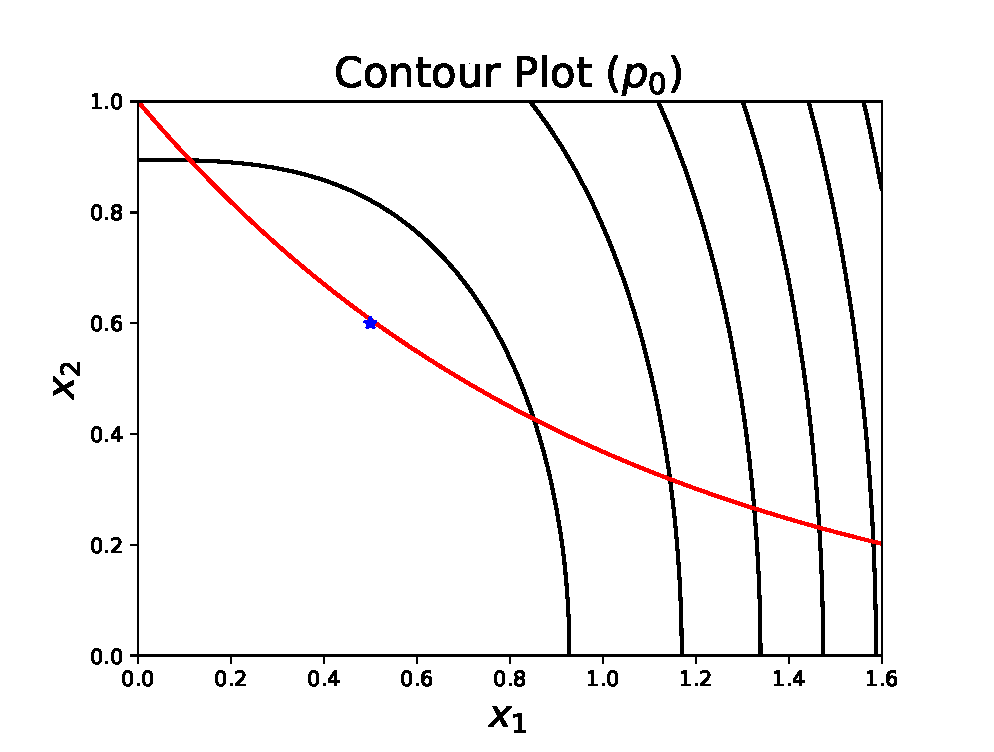
\includegraphics[scale=0.4]{Contour_p0}
		\end{minipage}
		\hspace{1cm}
		\begin{minipage}{0.4\textwidth}
			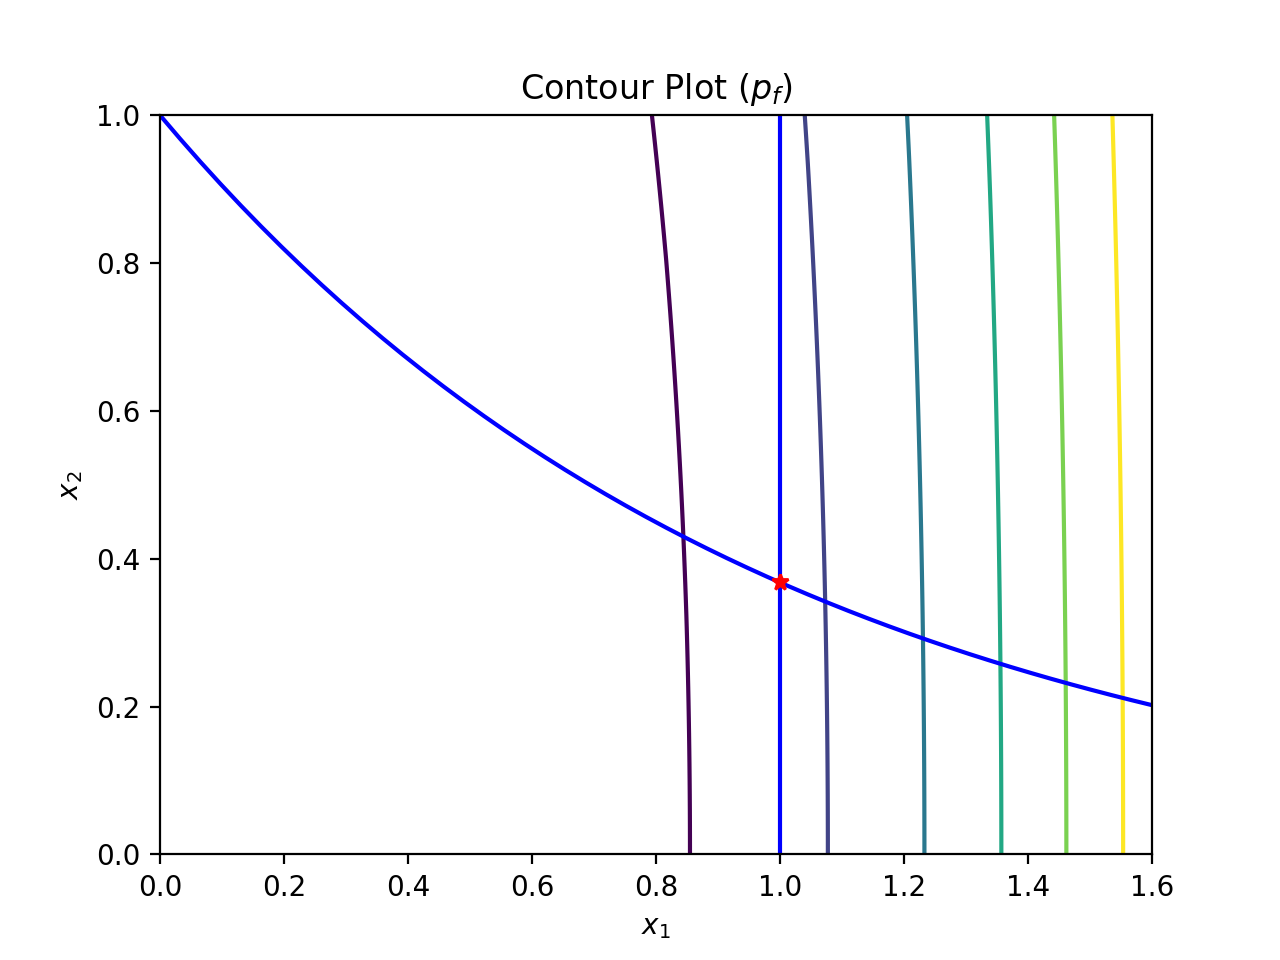
\includegraphics[scale=0.4]{Contour_pf}
		\end{minipage}
	\caption{Plot of the problem at $t=0$ and $t=1$}
	\label{fig:contour}
\end{figure}
The first thing to do before being able to apply any algorithm is to re-write the problem in the more standard NLP form:
\begin{mini}
	{x\in\mathbb{R}^2}{p_1x_1^3+x_2^2}{\label{eq:simple}}{}
	\addConstraint{e^{-x_1}-x_2\leq 0}{}
	\addConstraint{p_2-x_1\leq 0}{}
\end{mini}
We see that this problem has two inequality constraints ($n_{iq}=2$) and zero equality constraints ($n_{eq}=0$).
Algorithm \ref{alg:pathfollowing} is then applied to this problem which requires that the NLP to be solved to find the initial variables: $\boldsymbol{\chi}(\bf{p}_0),\boldsymbol{\lambda}^*(\bf{p}_0),\boldsymbol{\mu}^*(\bf{p}_0)$.
The NLP solution is then fed to a QP solver where the linearized NLP is solved as a QP.
Either the pure-predictor QP (\ref{eq:QP}) or the predictor-corrector QP (\ref{eq:QP_pc}) formulation can be used.
If the QP is feasible then the primal variables $\boldsymbol{\chi}$ are updated and the dual variables are updated either using the pure-predictor method or the predictor-corrector method depending on which QP was solved.
Next the step size is updated using the path following equation written previously.
If the QP is infeasible, then the step size is reduced and the QP is solved again.
\par
Figure \ref{fig:x1} illustrates how $x_1$ changes with respect to $t$ when $k=100$ iterations are used ($\Delta t = 0.01$).
The figure shows how $x_1$ changes steeply as the bound constraints become active.
\begin{figure}[H]
	\centering
	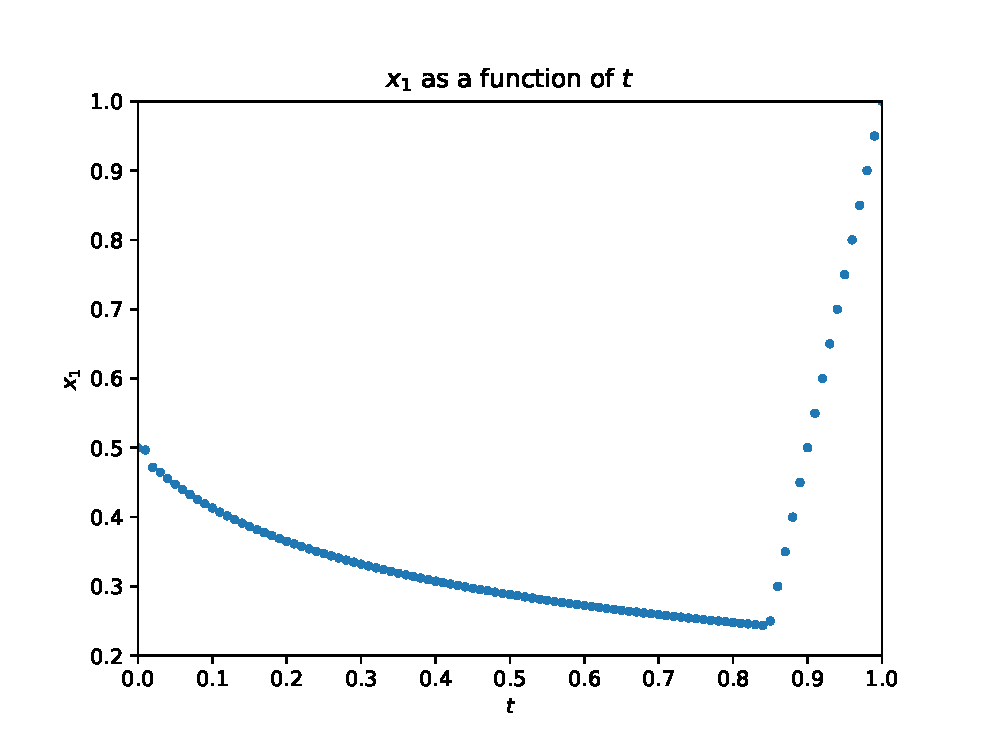
\includegraphics[scale=0.7]{x1}
	\caption{Plot of $x_1$ as a function of $t$, 100 iterations}
   \label{fig:x1}
\end{figure}
If less iterations are used, the final solution is still the same.
Figure \ref{fig:x1_2} illustrates $x_1$ versus time for $k=10$ iterations ($\Delta t=0.1$).
Notice that the shape of both the plots of $x_1$ versus time are the same and the final solution is still approximately the same.
\begin{figure}[H]
	\centering
	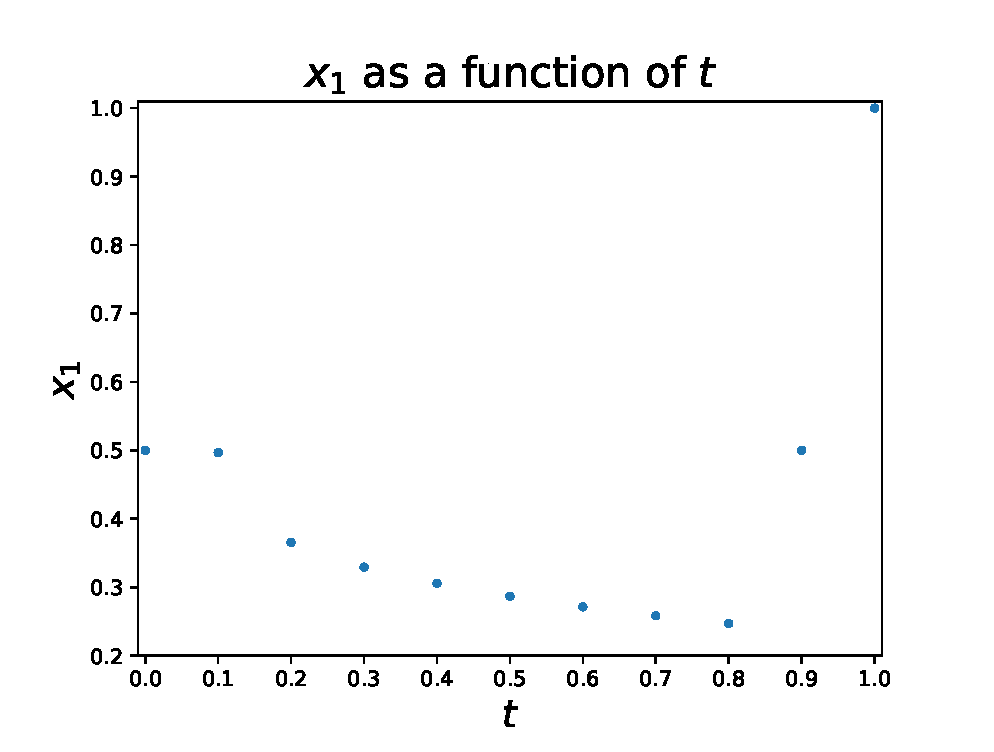
\includegraphics[scale=0.7]{x1_2}
	\caption{Plot of $x_1$ as a function of $t$, 10 iterations}
   \label{fig:x1_2}
\end{figure}
\par
While this is a simple problem, it is a good test for Algorithm \ref{alg:pathfollowing} since the problem changes substantially both in the nature of the active constraints and the slope of the objective function from $p_0$ to $p_f$\cite{param}.
\end{exmp}